\documentclass[12pt]{article}

\usepackage{amsfonts, amsmath, amssymb, amstext, latexsym}
\usepackage{graphicx, epsfig}
\usepackage[latin1]{inputenc}
\usepackage[french]{babel}
\usepackage{exscale}
\usepackage{amsbsy}
\usepackage{amsopn}
\usepackage{fancyhdr}

\newcommand{\noi}{\noindent}
\newcommand{\dsp}{\displaystyle}
\newcommand{\ind}{{{\large 1} \hspace*{-1.6mm} {\large 1}}}


\textheight 25cm
\textwidth 16cm
\oddsidemargin 0cm
\evensidemargin 0cm
\topmargin 0cm
\hoffset -0mm
\voffset -20mm


\pagestyle{plain}



% titre, auteur et date
\title{TP Principes et M\'{e}thodes Statistiques}
\author{Gabriel Sarrazin, Nejmeddine Douma, Simon Rabourg}
\date{Avril 2015}

% le debut du contenu
%===============
\begin{document}
%===============

% pour afficher titre, auteur et date
\maketitle

\section{Analyse des d\'{e}fauts de cuves}


\section{V\'{e}rifications exp\'{e}rimentales \`{a} base de simulations}


\begin{enumerate}
\item Il est possible de simuler n \'{e}chantillons de la loi Pa(a,b) car nous connaissons sa fonction de r\'{e}partiton. 
\\
$P_a(a,b)$ est une fonction continue, elle peut donc s'apparenter \`{a} une loi uniforme.  Dans un premier temps, simuler n \'{e}chantillons de cette loi va donc consister  \`{a} tirer, au hasard, n valeurs al\'{e}atoires sur l'intervalle [0,1]. Connaissant la fonction de r\'{e}partition de la loi  $P_a(a,b)$,nous allons ensuite calculer l'image inverse $ F^{-1}(Ui)$ pour obtenir un \'{e}chantillon de loi $P_a(a,b)$ et nous ferons selons cela pour les n valeurs obtenues sur [0,1]
\\
Nous pouvons repr\'{e}senter cette m\'{e}thode sous forme d'un graphique : en mettant en ordonn\'{e}e les n valeurs de la loi Ui et en abscisse la projection pour chacune de ses valeurs de son image inverse ($F^{-1}(Ui)$ ).
\\

\item
 En suivant la m\'{e}thode d\'{e}crite pr\'{e}cedemment, nous  avons simuler m \'{e}chantillon de taille n avec diff\'{e}rentes valeurs pour m,n et a. 


\begin{figure*}[ht]
\label{graph1}
\centering
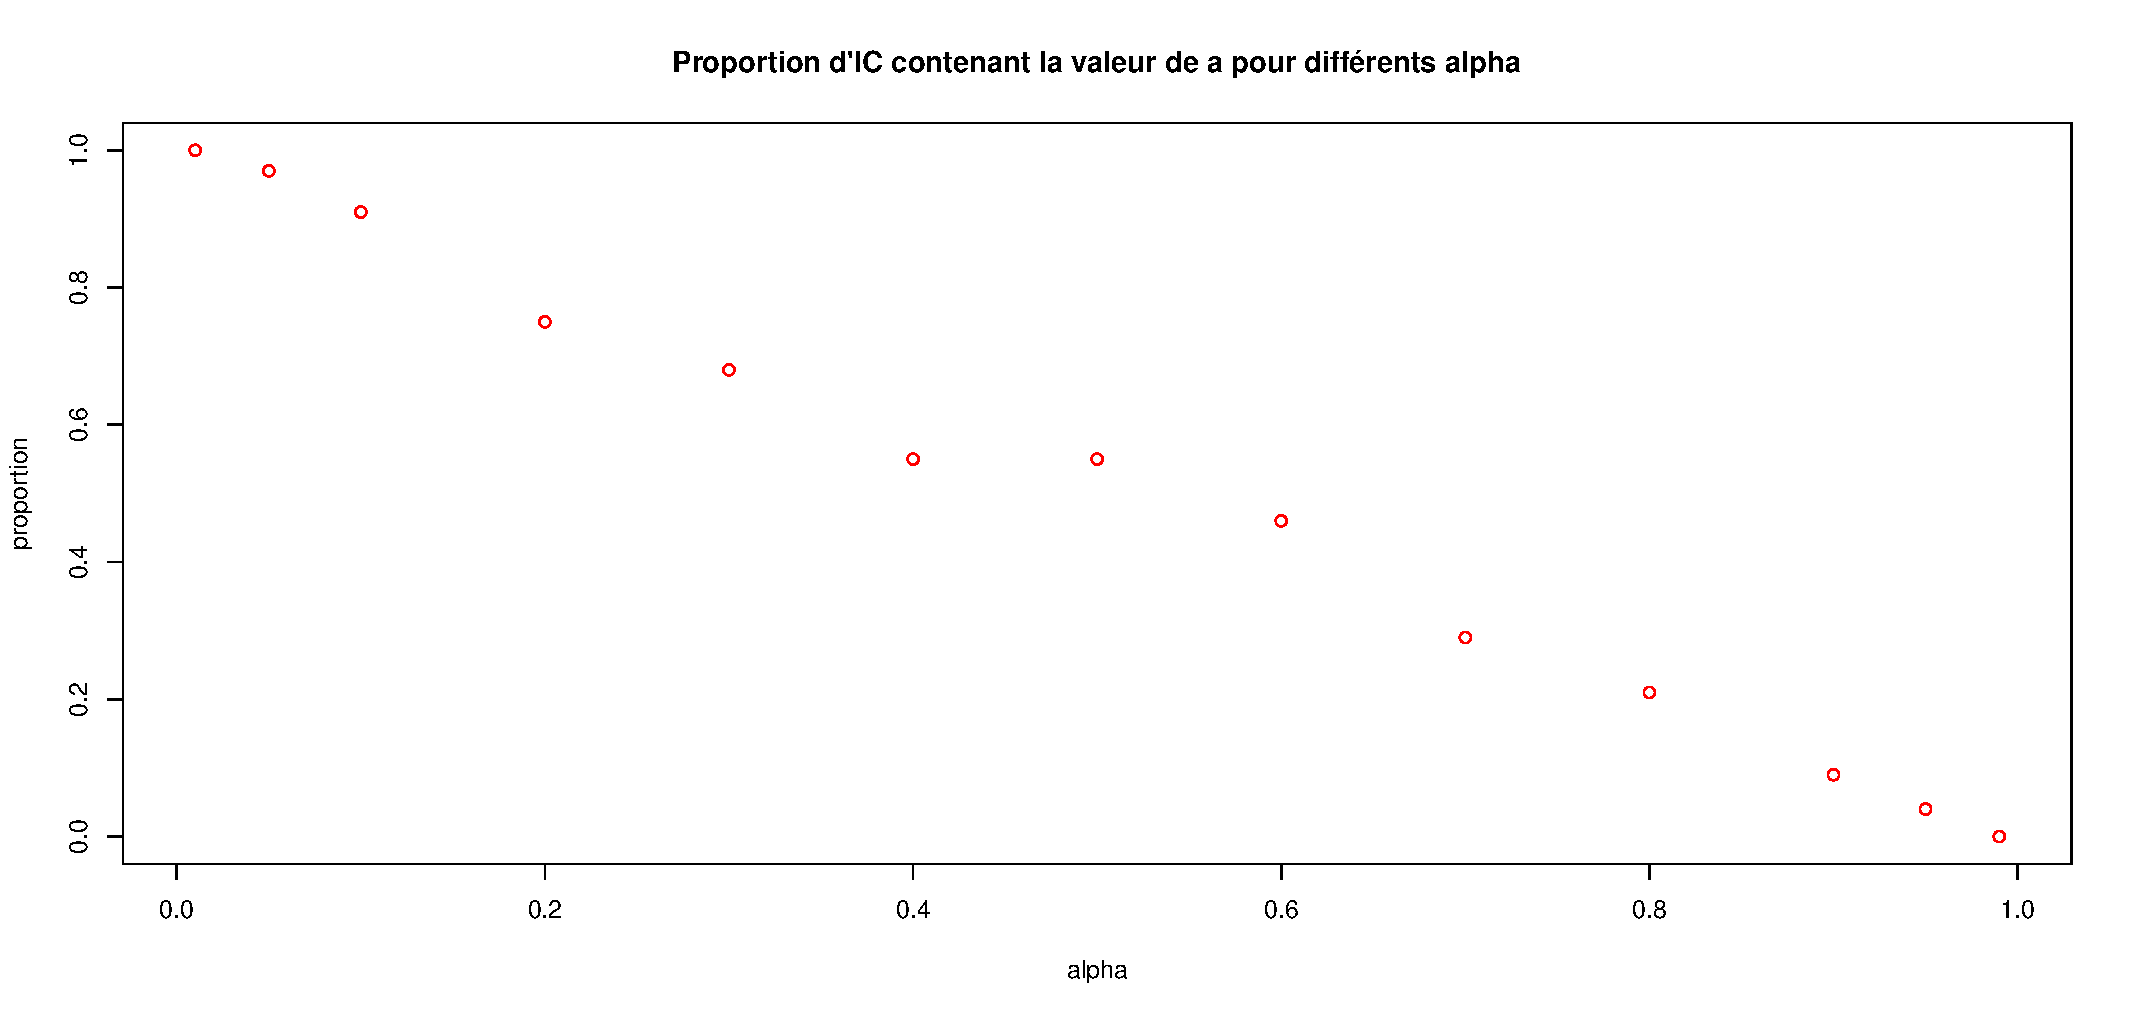
\includegraphics[width=1.0\textwidth]{figures/Graph_P2Q2.pdf}
\caption{Graphe des proportions d'IC($\alpha$) contenant la valeur exacte de a pour diff\'{e}rentes valeurs de $\alpha$}
\end{figure*}


Nous avons ensuite, pour chaque \'{e}chantillon de taille n, calculer l'intervalle de confiance bilat\'{e}ral. Pour cela nous avons utiliser L'intervalle de confiance trouv\'{e} en premi\`{e}re partie qui s'utilise avec $Y=\ln {\dsp \frac{X}{2}}$.  A chaque fois que a est bien contenu dans cet intervalle, nous inc\'{e}mentons une variable compteur. La proportion Pr d'IC contenant a est donc $Pr = Compteur/m$.
\\
Afin que cela soit plus repr\'{e}sentatif,nous avons trac\'{e} un graphique avec les diff\'{e}rentes proportions obtenues en fonction des $\alpha$. (Voir figure page \ref{graph1})
\\

Nous pouvons voir qu'il existe une lin\'{e}arit\'{e} entre la proportion et les $\alpha$. Plus on augmente le nombre d'\'{e}chantillon m et leur taille n et plus l'approximation est exacte. Ces points ont \'{e}t\'{e} obtenus pour les valeurs de $m = 100$, $n = 10, 30, 50, 100, 200, 500$, $a = 3, 5, 10, 20, 50$ et $\alpha = 0.01, 0.05, 0.10, 0.20 ..., 0.80, 0.90, 0.95, 0.99$.
\\
Quand on simule un grand nombre m d\'{e}chantillons de taille $n$ de la  loi $P_a(a,2)$ alors la proportion d'IC($\alpha$) contenant $a$ est aproximativement \'{e}gale \`{a}  $1 - \alpha$.
\\

\item Afin d'\'{e}stimer le param\`{e}tre $a$, nous disposons de trois m\'{e}thodes : la m\'{e}thodes des moments, la m\'{e}thode du maximum de vraisemblance qui nous m\`{e}nent au m\^{e}me r\'{e}sultat pour l'\'{e}stimation du param\`{e}tre $a$ et nous pouvons aussi d\'{e}terminer l'\'{e}stimateur sans bais de variance minimale si celui-ci existe.
\\
Pour chaque \'{e}chantillons (m en tout) nous mis au point sur R une fonction qui calcule les estimateurs propos\'{e}s , qui estime le biais et l'erreur quadratique de chaque estimateur, et qui fait une moyenne pour chacun de ces r\'{e}sultats. Par ces r\'{e}sultats, nous pouvons tracer un histogramme des estimateurs obtenus avec en rouge : la moyenne de ces estimateurs et en bleu : la valeur exacte de a pour laquelle il faut \^{e}tre la plus proche.
\\

Pour chaque graphique voici les moyennes des biais et des EQM obtenus pour chaque estimateur:
\begin{itemize}
\item Moyenne des biais EMV 1.691318 
Moyenne des biais ESBVM -0.6469459 
Moyenne des EQM EMV 38.3953 
Moyenne des EQM ESBVM 23.16078 
\item Moyenne des biais EMV 0.7355605 
Moyenne des biais ESBVM 0.1987825 
Moyenne des EQM EMV 6.691049 
Moyenne des EQM ESBVM 5.589889 
\item Moyenne des biais EMV 0.08228447 
Moyenne des biais ESBVM -0.1193612 
Moyenne des EQM EMV 1.867297 
Moyenne des EQM ESBVM 1.801097 
\item Moyenne des biais EMV 0.1657237 
Moyenne des biais ESBVM 0.06406643 
Moyenne des EQM EMV 0.8215394 
Moyenne des EQM ESBVM 0.7823774 
\item Moyenne des biais EMV 0.02238977 
Moyenne des biais ESBVM 0.002344989 
Moyenne des EQM EMV 0.207069 
Moyenne des EQM ESBVM 0.2057478 
\\
\end{itemize}


Apr\`{e}s analyse des r\'{e}sultats et des graphiques, nous pouvons en d\'{e}duire que le meilleur estimateur est l'$ESBVM$ car il poss\`{e}de  le biais et l'erreur quadratique moyenne le plus faible sur l'ensemble des \'{e}chantillons. Il faut noter que plus la taille des \'{e}chantillons est \'{e}lev\'{e}e, plus les estimateurs sont pr\'{e}cis. Nous pouvons tout de m\^{e}me constater que quelque soit le taille de l'\'{e}chantillon, l'$ESBVM$ est le meilleur estimateur.
\\
\begin{figure*}[ht]
\centering
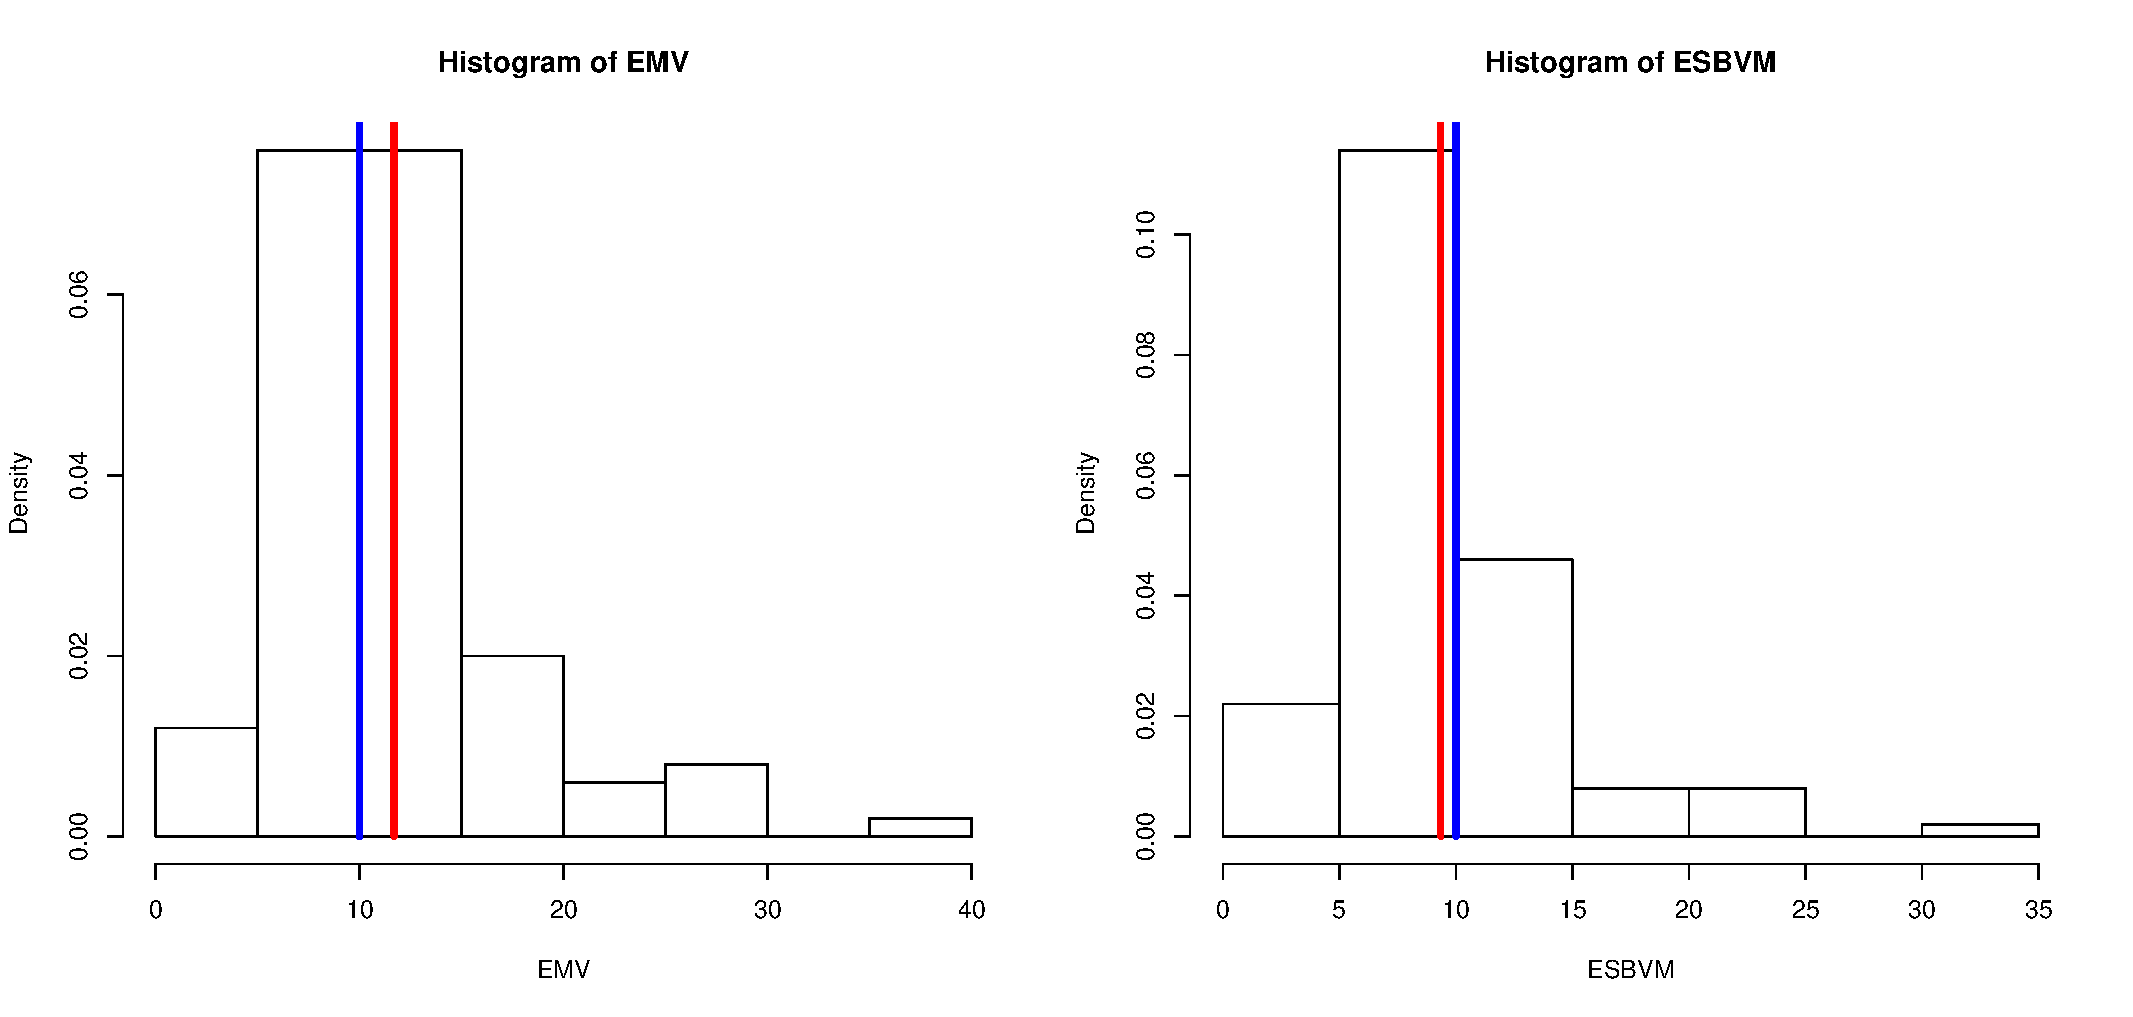
\includegraphics[width=1.0\textwidth]{figures/GraphP2Q31.pdf}
\caption{Histogramme des EMV et ESBVM pour $m=100, n=5, a=10$}
\end{figure*}

\begin{figure*}[ht]
\centering
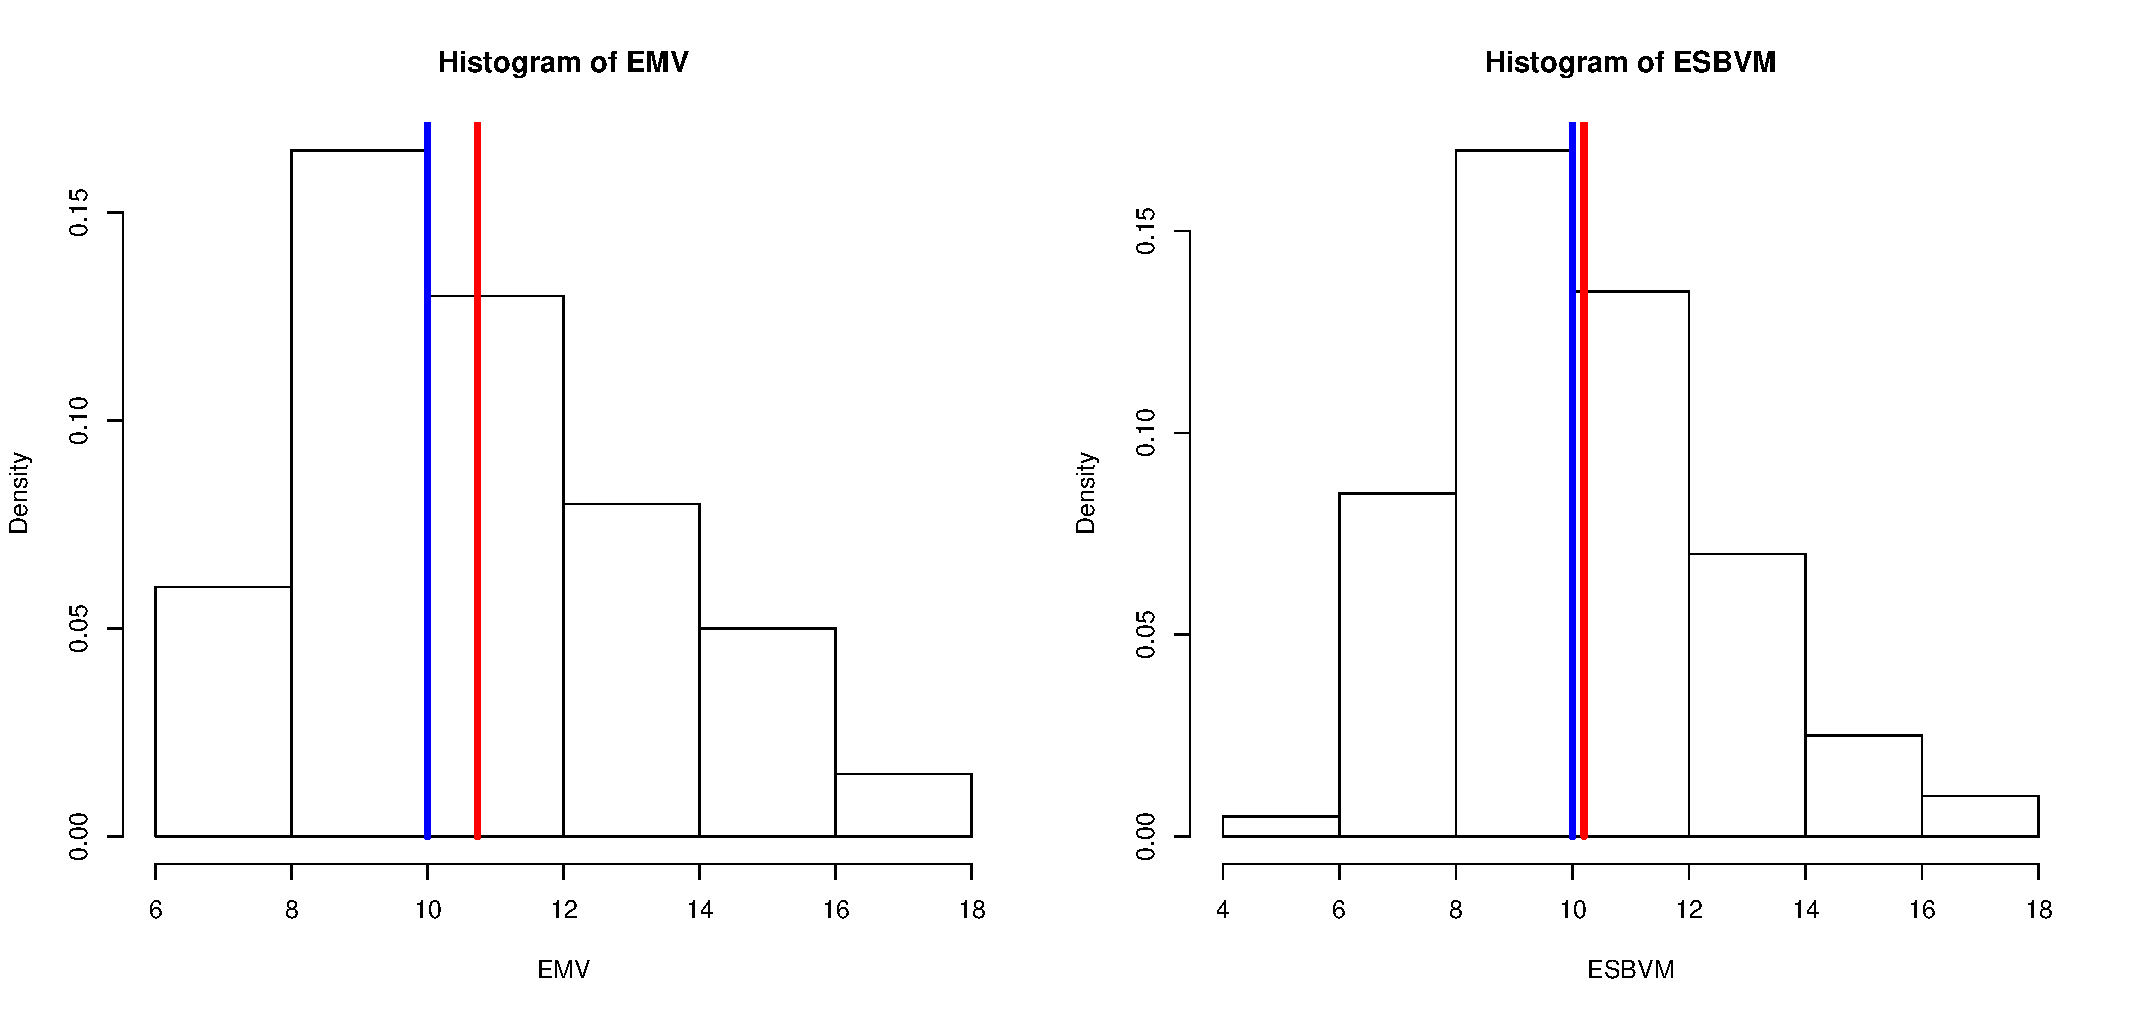
\includegraphics[width=1.0\textwidth]{figures/GraphP2Q32.pdf}
\caption{Histogramme des EMV et ESBVM pour $m=100, n=20,   a=10$}
\end{figure*}

\begin{figure*}[ht]
\centering
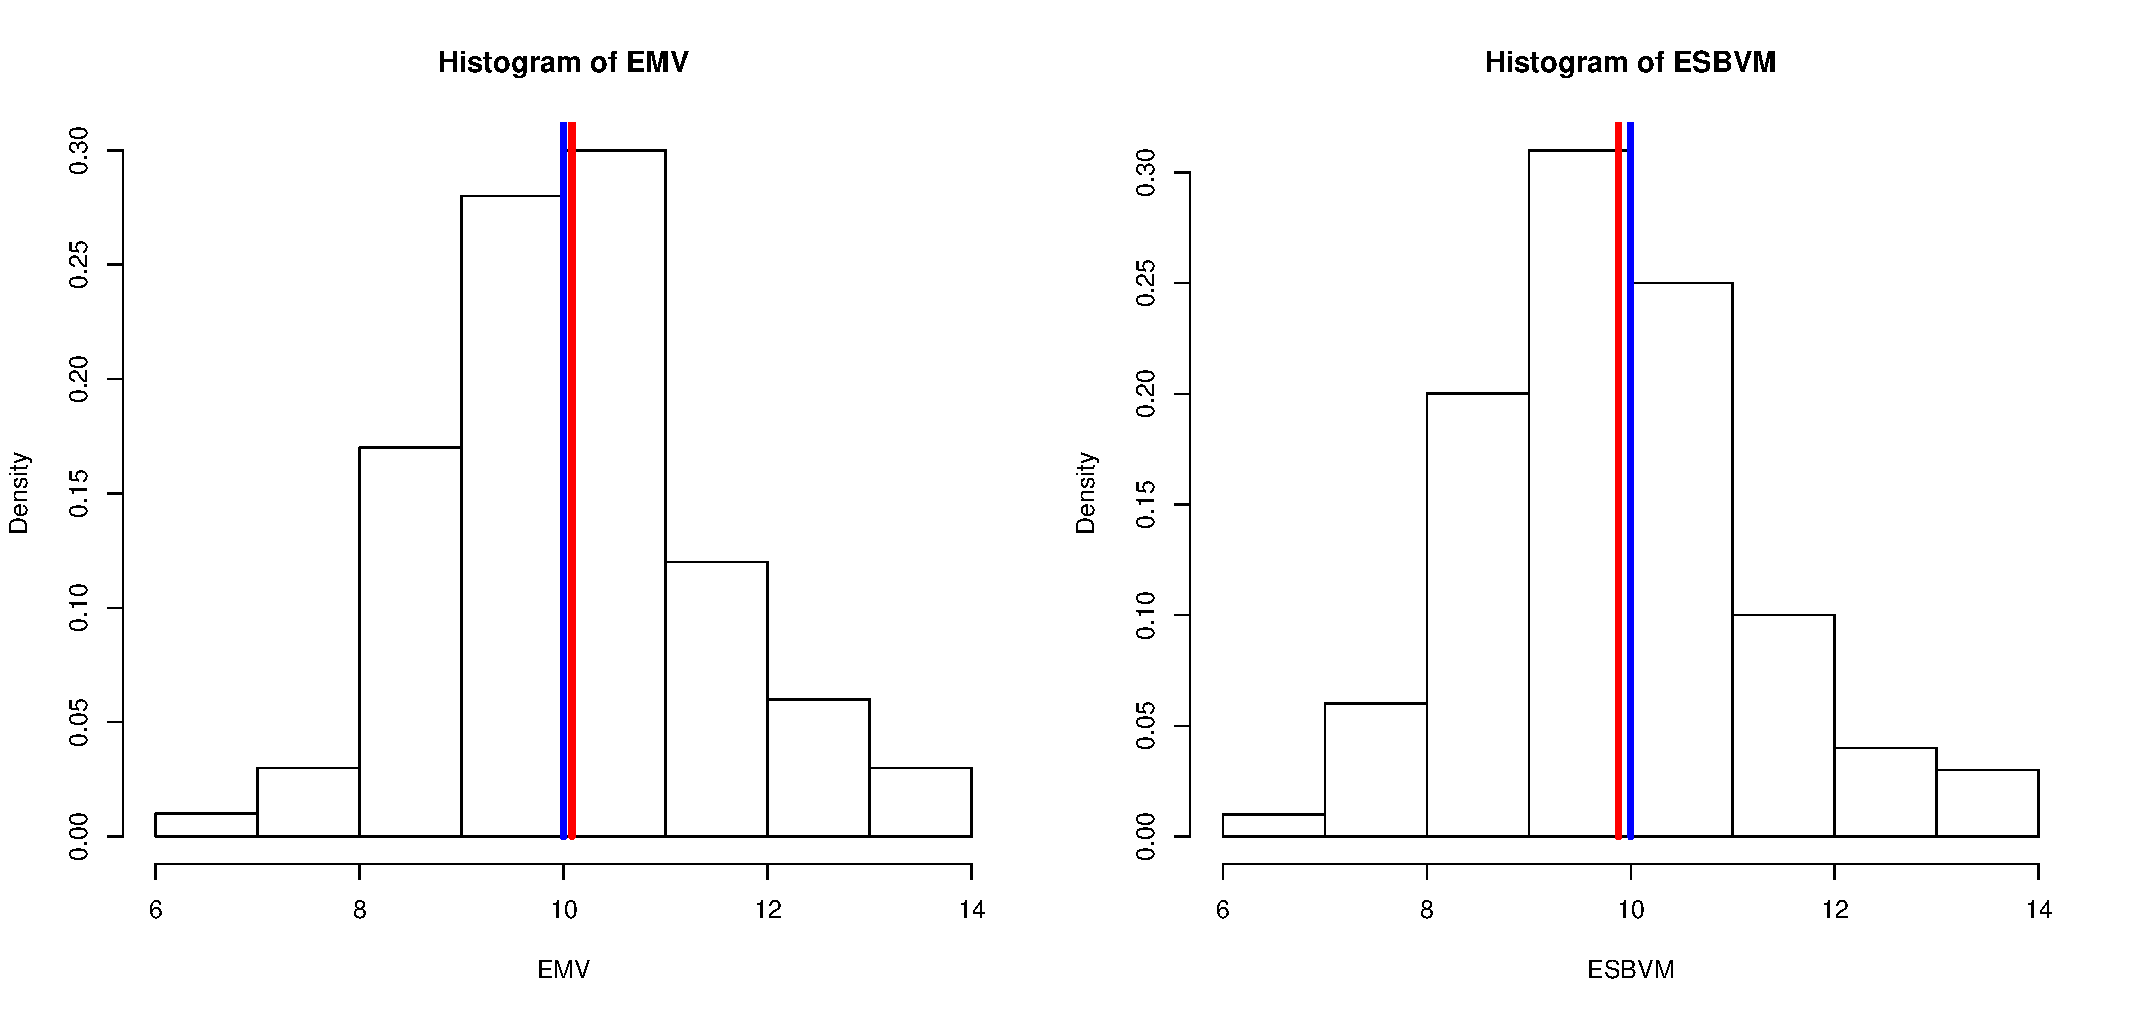
\includegraphics[width=1.0\textwidth]{figures/GraphP2Q33.pdf}
\caption{Histogramme des EMV et ESBVM pour $m=100, n=50, a=10$}
\end{figure*}

\begin{figure*}[ht]
\centering
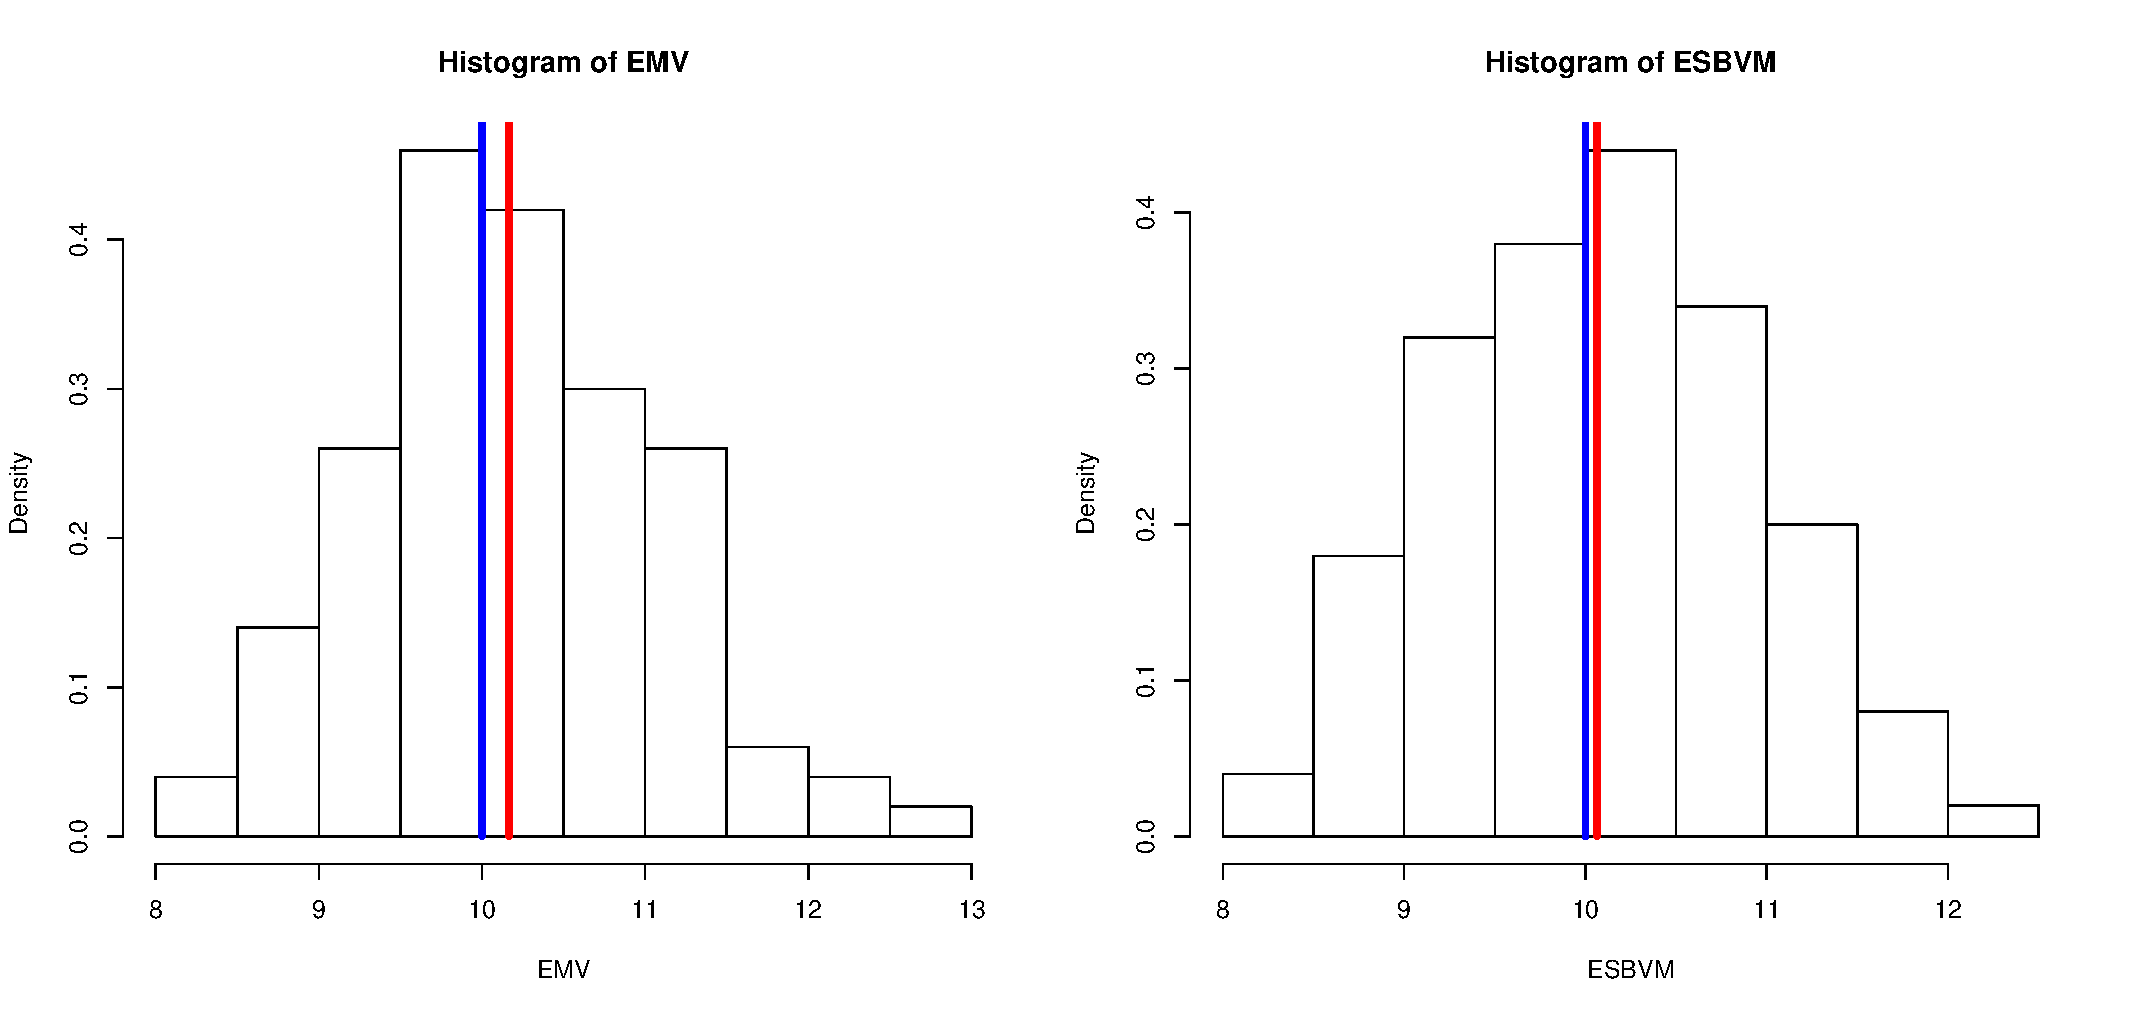
\includegraphics[width=1.0\textwidth]{figures/GraphP2Q34.pdf}
\caption{Histogramme des EMV et ESBVM pour $m=100, n=100, a=10$}
\end{figure*}

\begin{figure*}[ht]
\centering
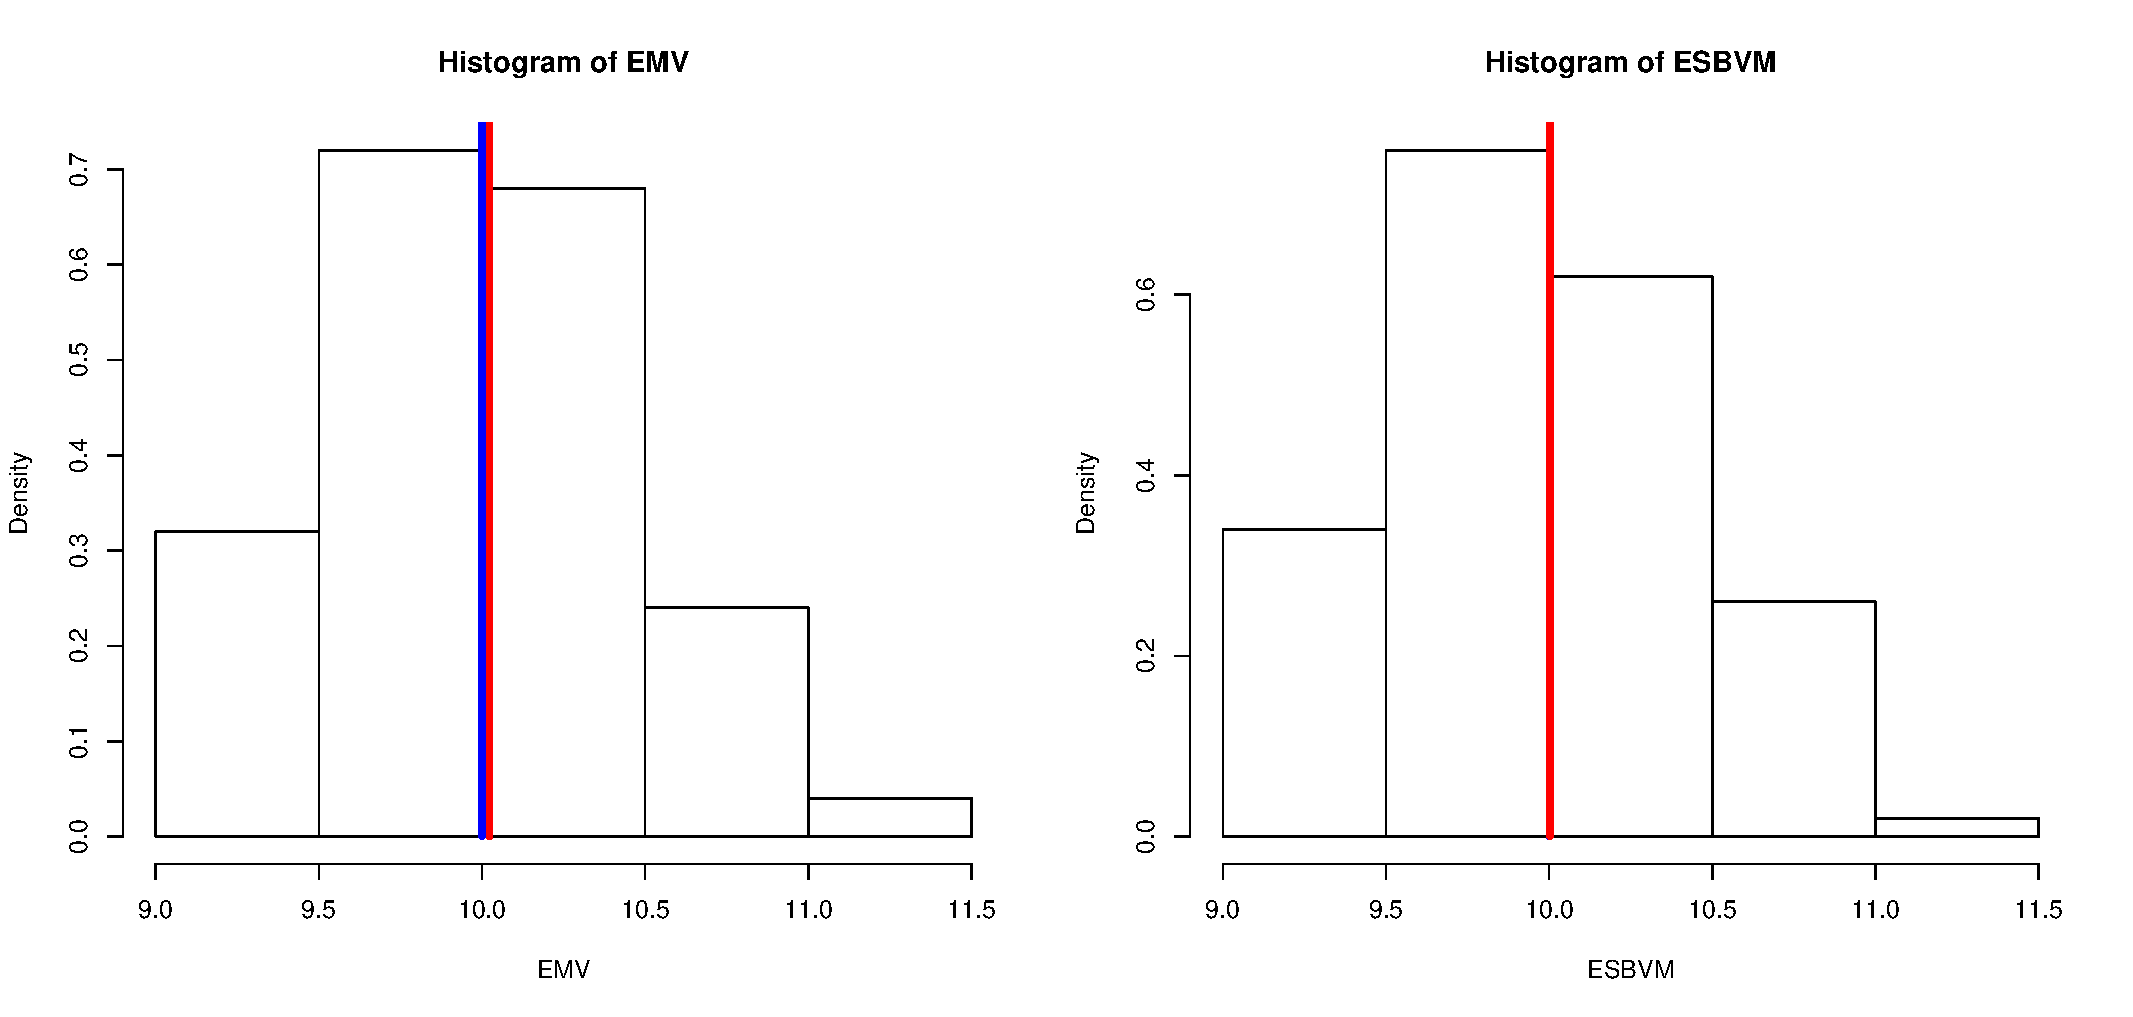
\includegraphics[width=1.0\textwidth]{figures/GraphP2Q35.pdf}
\caption{Histogramme des EMV et ESBVM pour $m=500, n=5, a=10$}
\end{figure*}

\begin{figure*}[ht]
\label{graphe2}
\centering
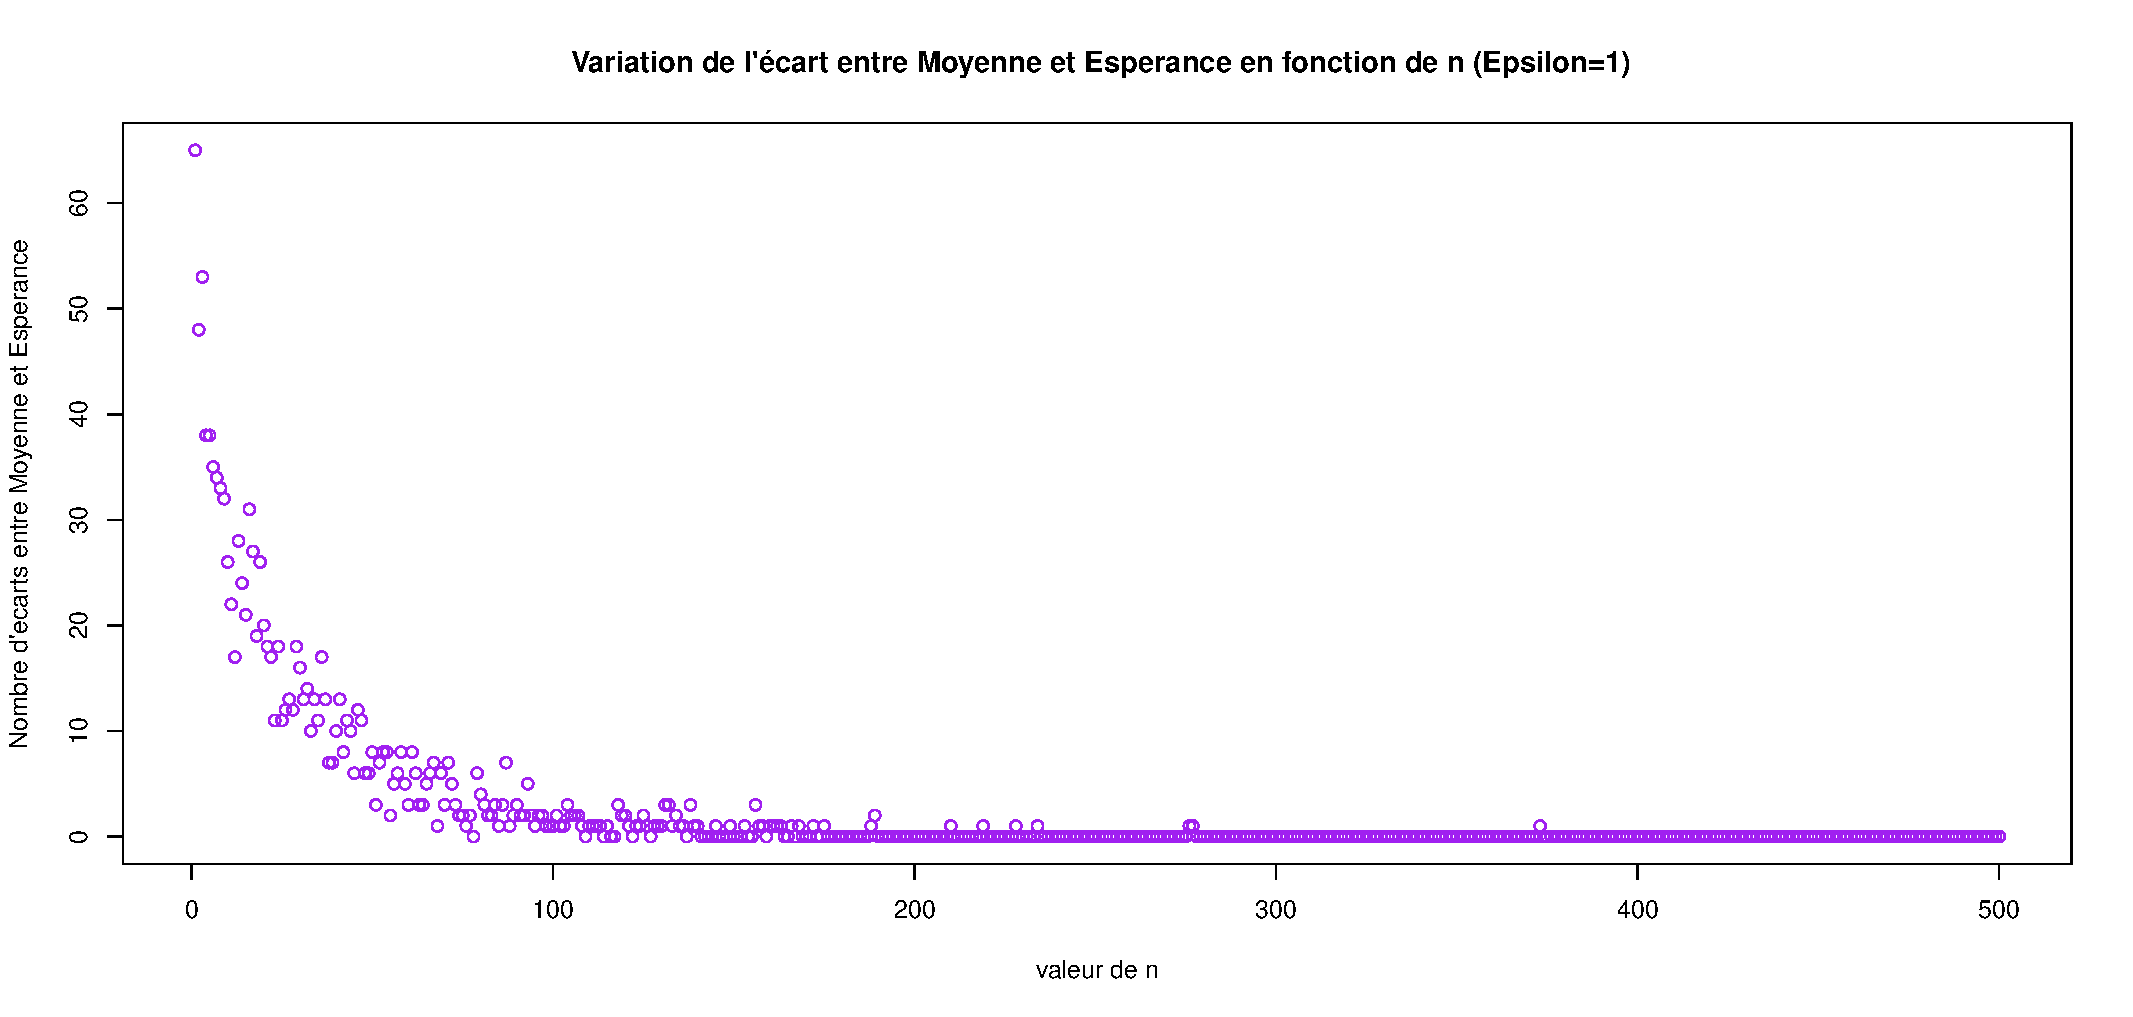
\includegraphics[width=1.0\textwidth]{figures/GraphP2Q4.pdf}
\caption{Variation de la diff\'{e}rence absolue entre Moyenne est Esperance en fonction de n }
\end{figure*}

\item
Dans cette partie nous simulons \`{a} nouveau m \'{e}chantillons de taille n suivant la loi $P_a(a,2)$ . Nous calculons la moyenne empirique \`{a}  l'aide de la fonction $mean$ disponible sur R et nous calculons son Esperance. Pour chaque valeur n allant de 5 \`{a}  500 nous calculons la difference absolue de ces deux param\`{e}tres. Nous avons ensuite enregistrer le nombre de fois o\`{u} la valeur d\'{e}passe une valeur $\epsilon (Ici, \epsilon = 1 )$. Sur la figure qui suit (page \ref{graphe2}, nous pouvons remarquer que plus la taille de  l'\'{e}chantillon grandit, moins la diff\'{e}rence entre la moyenne et l'esperance de cet \'{e}chantillon est grande.
\\
Par cons\'{e}quent, plus n est grand, moins la moyenne empirique $\bar X_n$  s'\'{e}loigne de l'Esperance $E(X)$ d'au moins $\epsilon$.
On a donc $$\forall\varepsilon>0,\quad \lim_{n \to +\infty} \mathbb{P}\left(\left|\frac{X_1+X_2+\cdots+X_n}{n} -E(X)\right| \geqslant \varepsilon\right) = 0 $$

Autrement dit, $(X_n)$ converge en probabilit\'{e} vers $E(X)$. La moyenne empirique est bien un estimateur convergent de l'\'{e}sperance.

\item
Apr\`{e}s avoir simuler m \'{e}chantillons de taille n suivant la loi $P_a(a,2)$, nous calculons leur moyenne. Nous obtenons donc un \'{e}chantillon de  moyennes empiriques. Pour diff\'{e}rente valeurs de n (Voir figures), nous avons trac\'{e} un histogramme et un graphe de la probabilit\'{e}s pour la loi normale  \`{a} l'aide de la function R $qqnorm$ qui permet de comparer graphiquement la distribution de l'\'{e}chantillon des m moyennes empiriques avec une distribution normale.
\\
Nous pouvons constater que pour $n=5$ il est difficile de dire que la loi normale est un mod\`{e}le approri\'{e}. Cependant, plus n augmente et plus les point sont align\'{e}s. 
\\ 
Nous pouvons donc en d\'{e}duire que pour n "suffisamment" grand, la loi de $\bar X_n$ est approximativement une loi normale.
\begin{figure*}[ht]
\centering
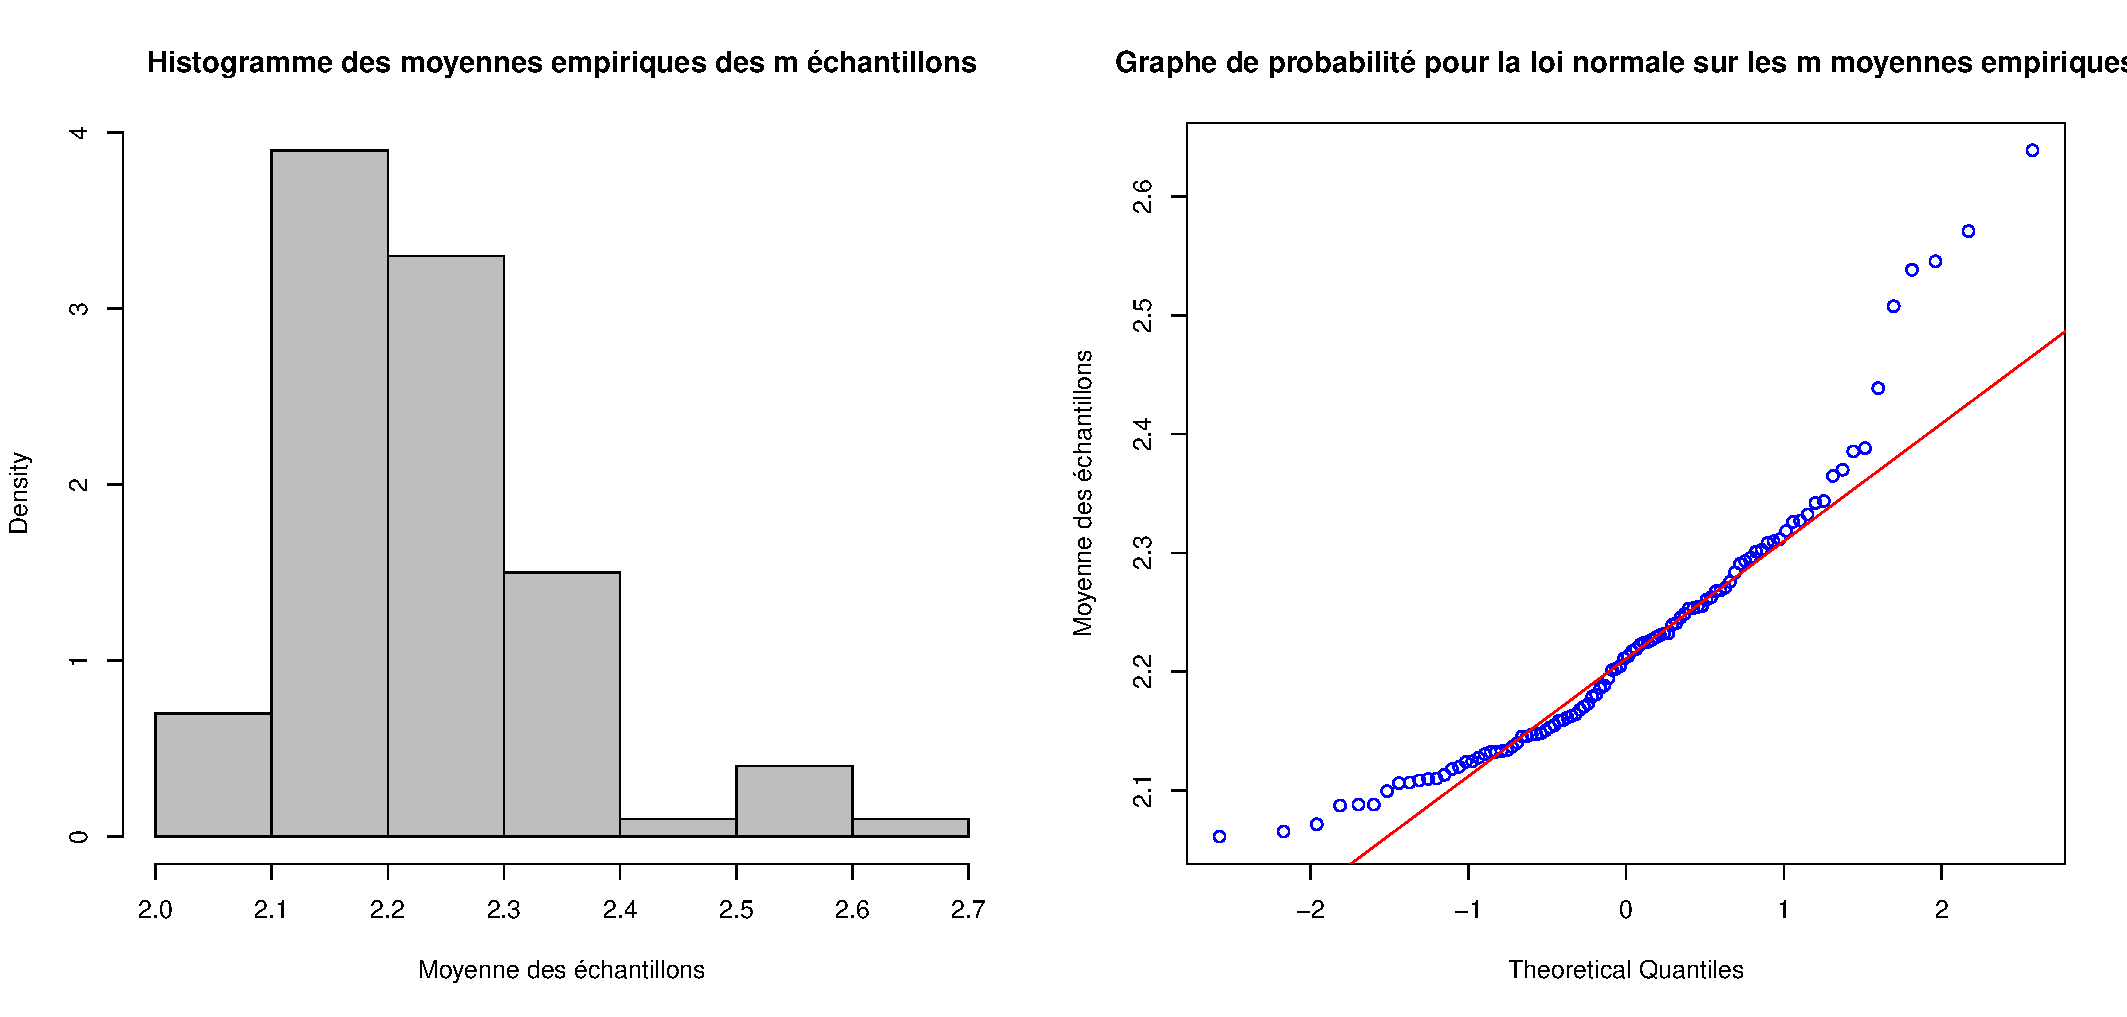
\includegraphics[width=1.0\textwidth]{figures/GraphP2Q51.pdf}
\caption{Etude de la distribution $\bar X_n$ par une distribution normale pour n=5}
\end{figure*}

\begin{figure*}[ht]
\centering
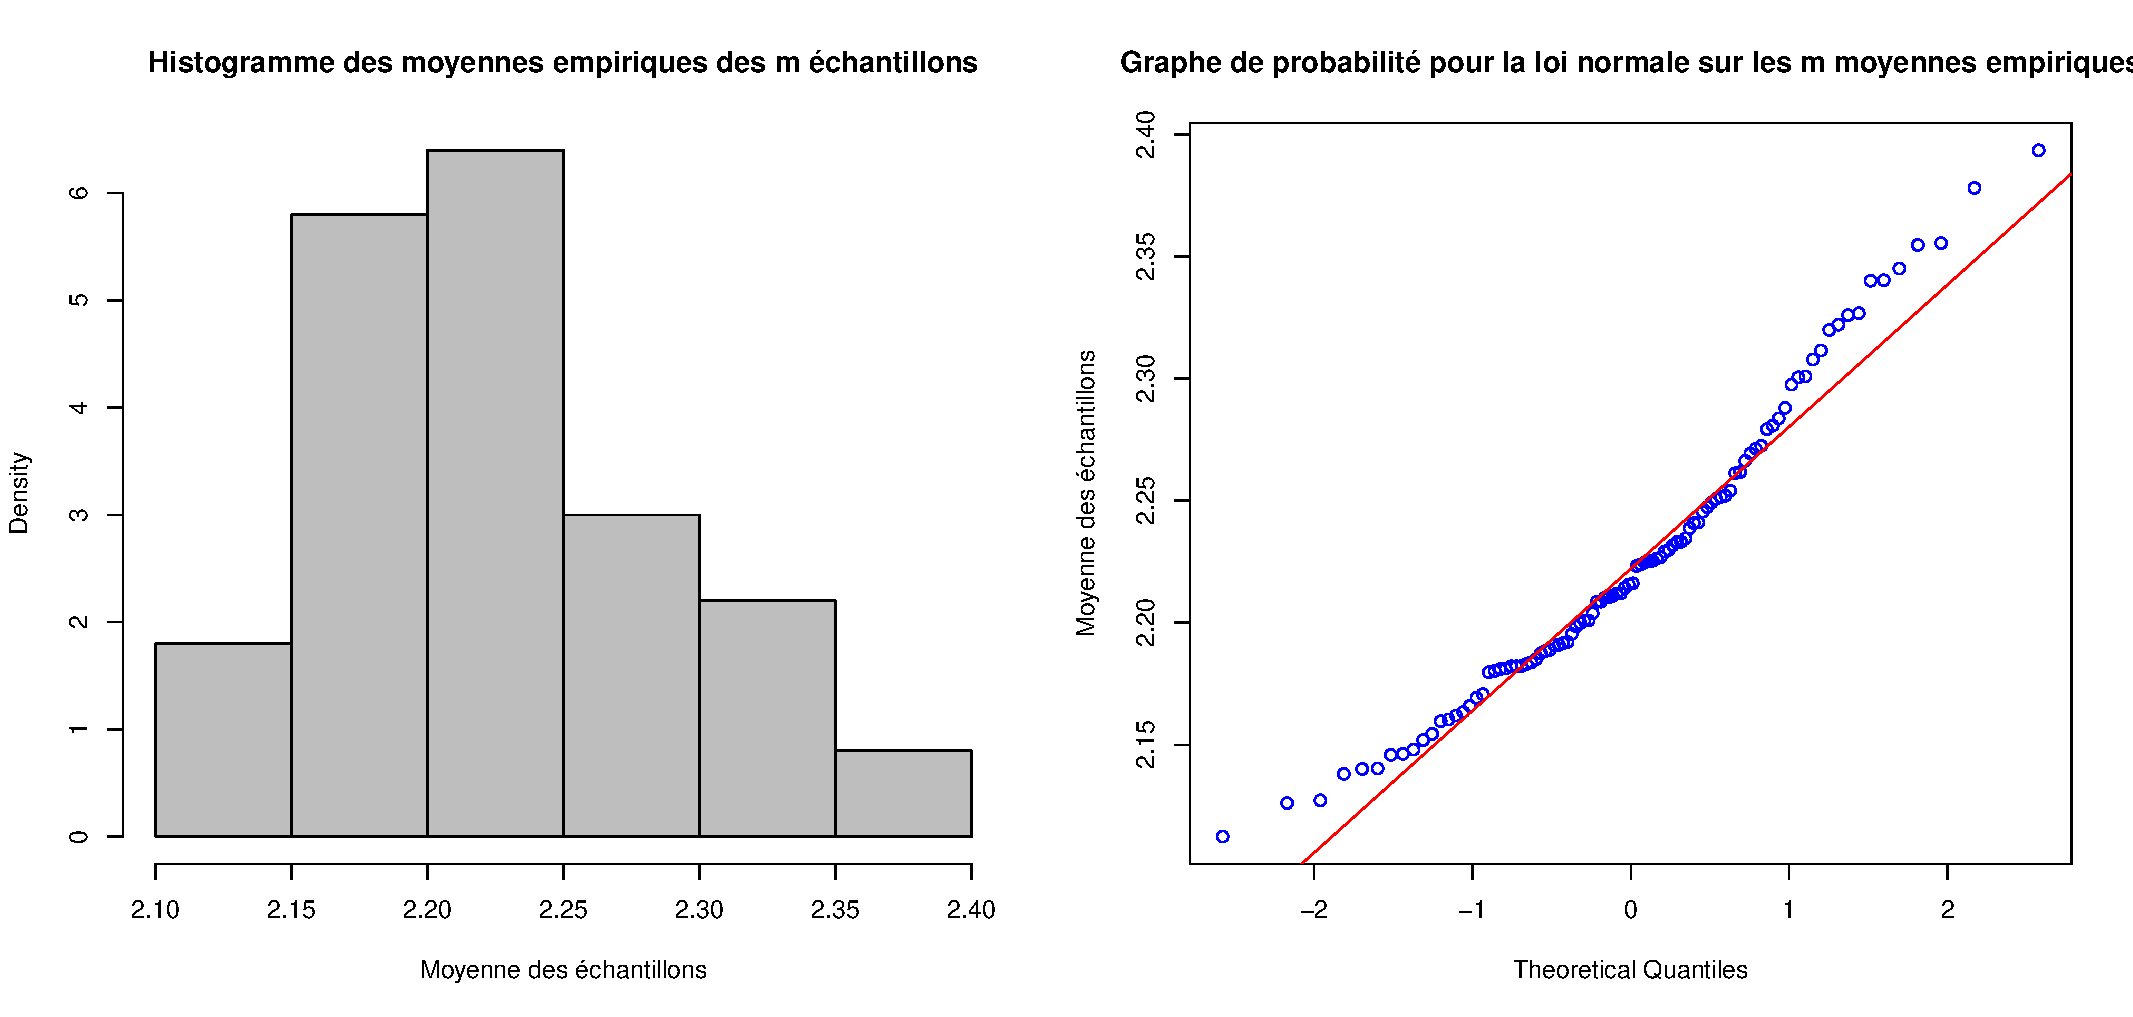
\includegraphics[width=1.0\textwidth]{figures/GraphP2Q52.pdf}
\caption{Etude de la distribution $ \bar X_n$ par une distribution normale pour n=10}
\end{figure*}

\begin{figure*}[ht]
\centering
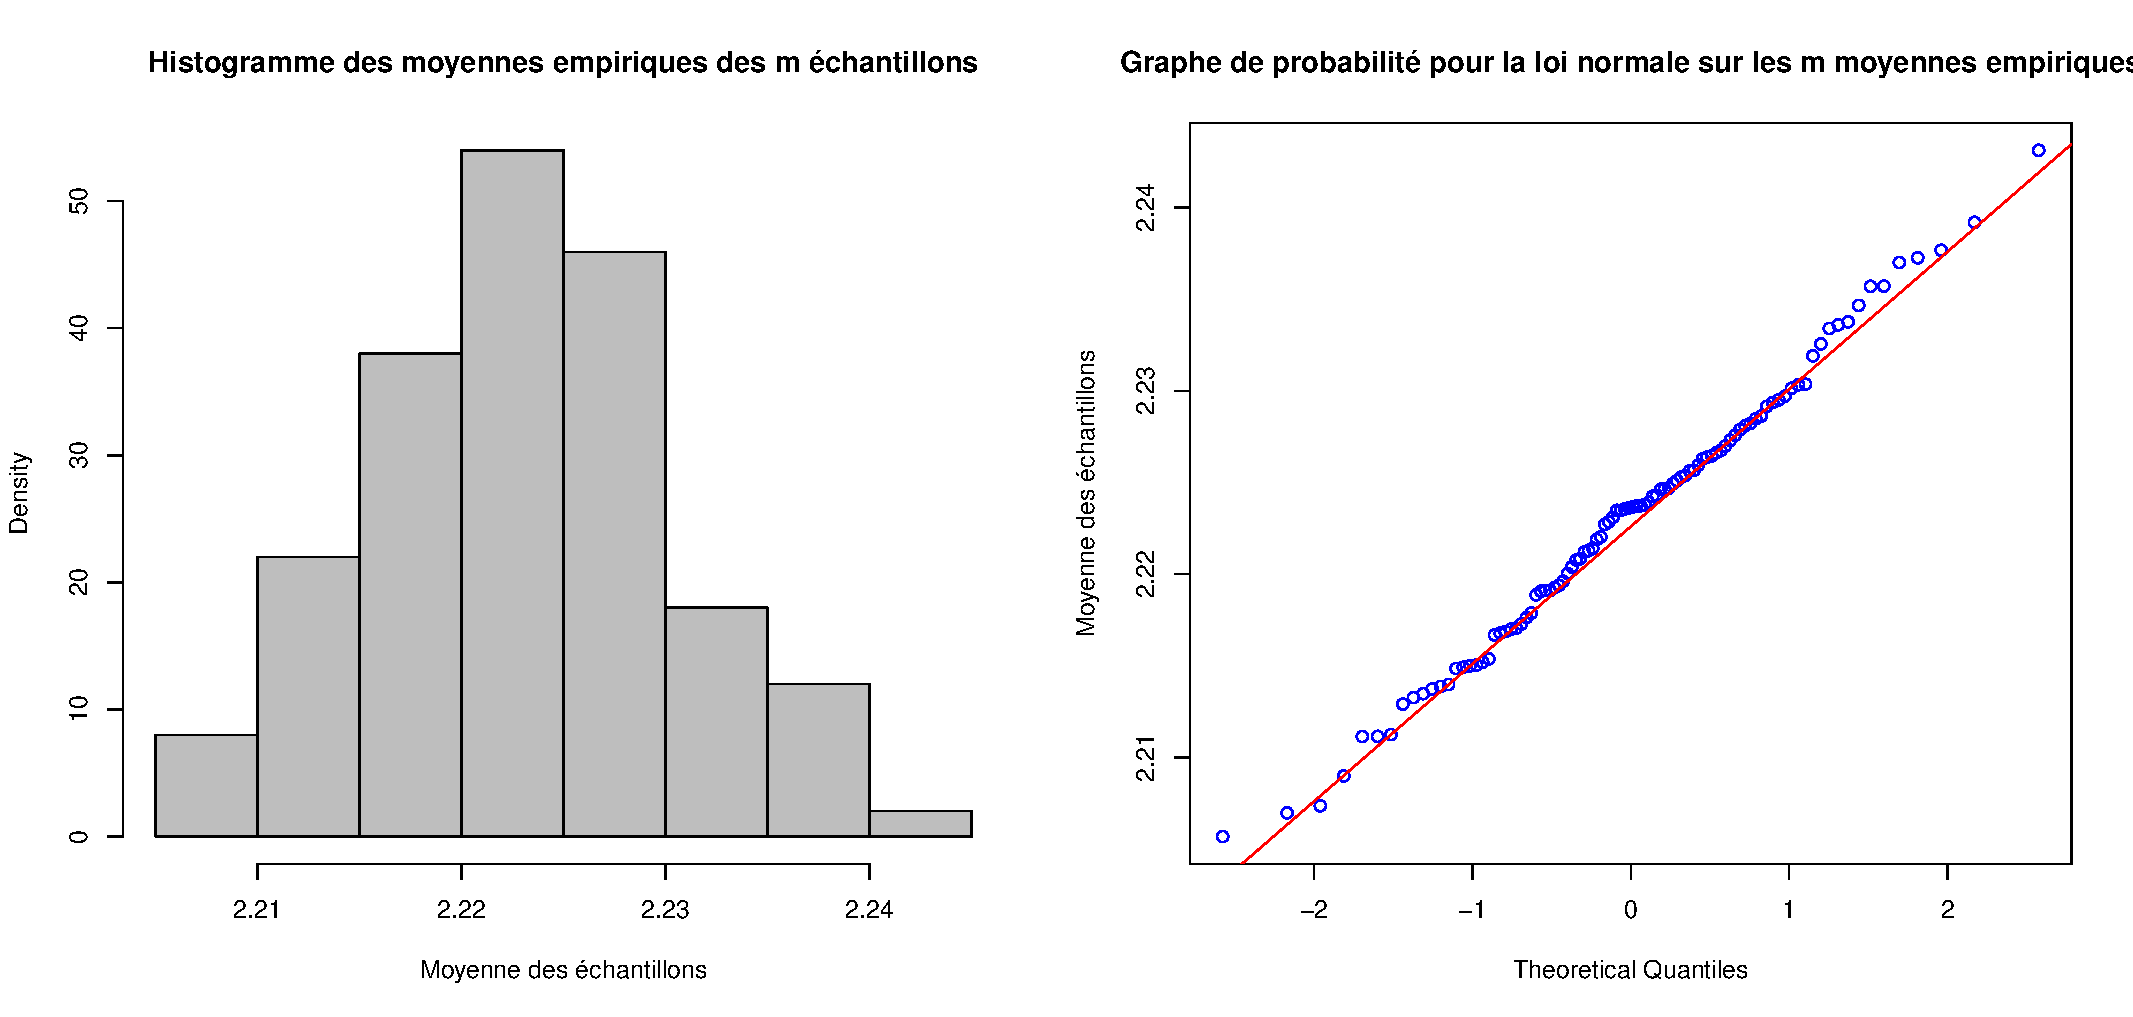
\includegraphics[width=1.0\textwidth]{figures/GraphP2Q53.pdf}
\caption{Etude de la distribution $\ bar X_n$ par une distribution normale pour n=50}
\end{figure*}

\begin{figure*}[ht]
\centering
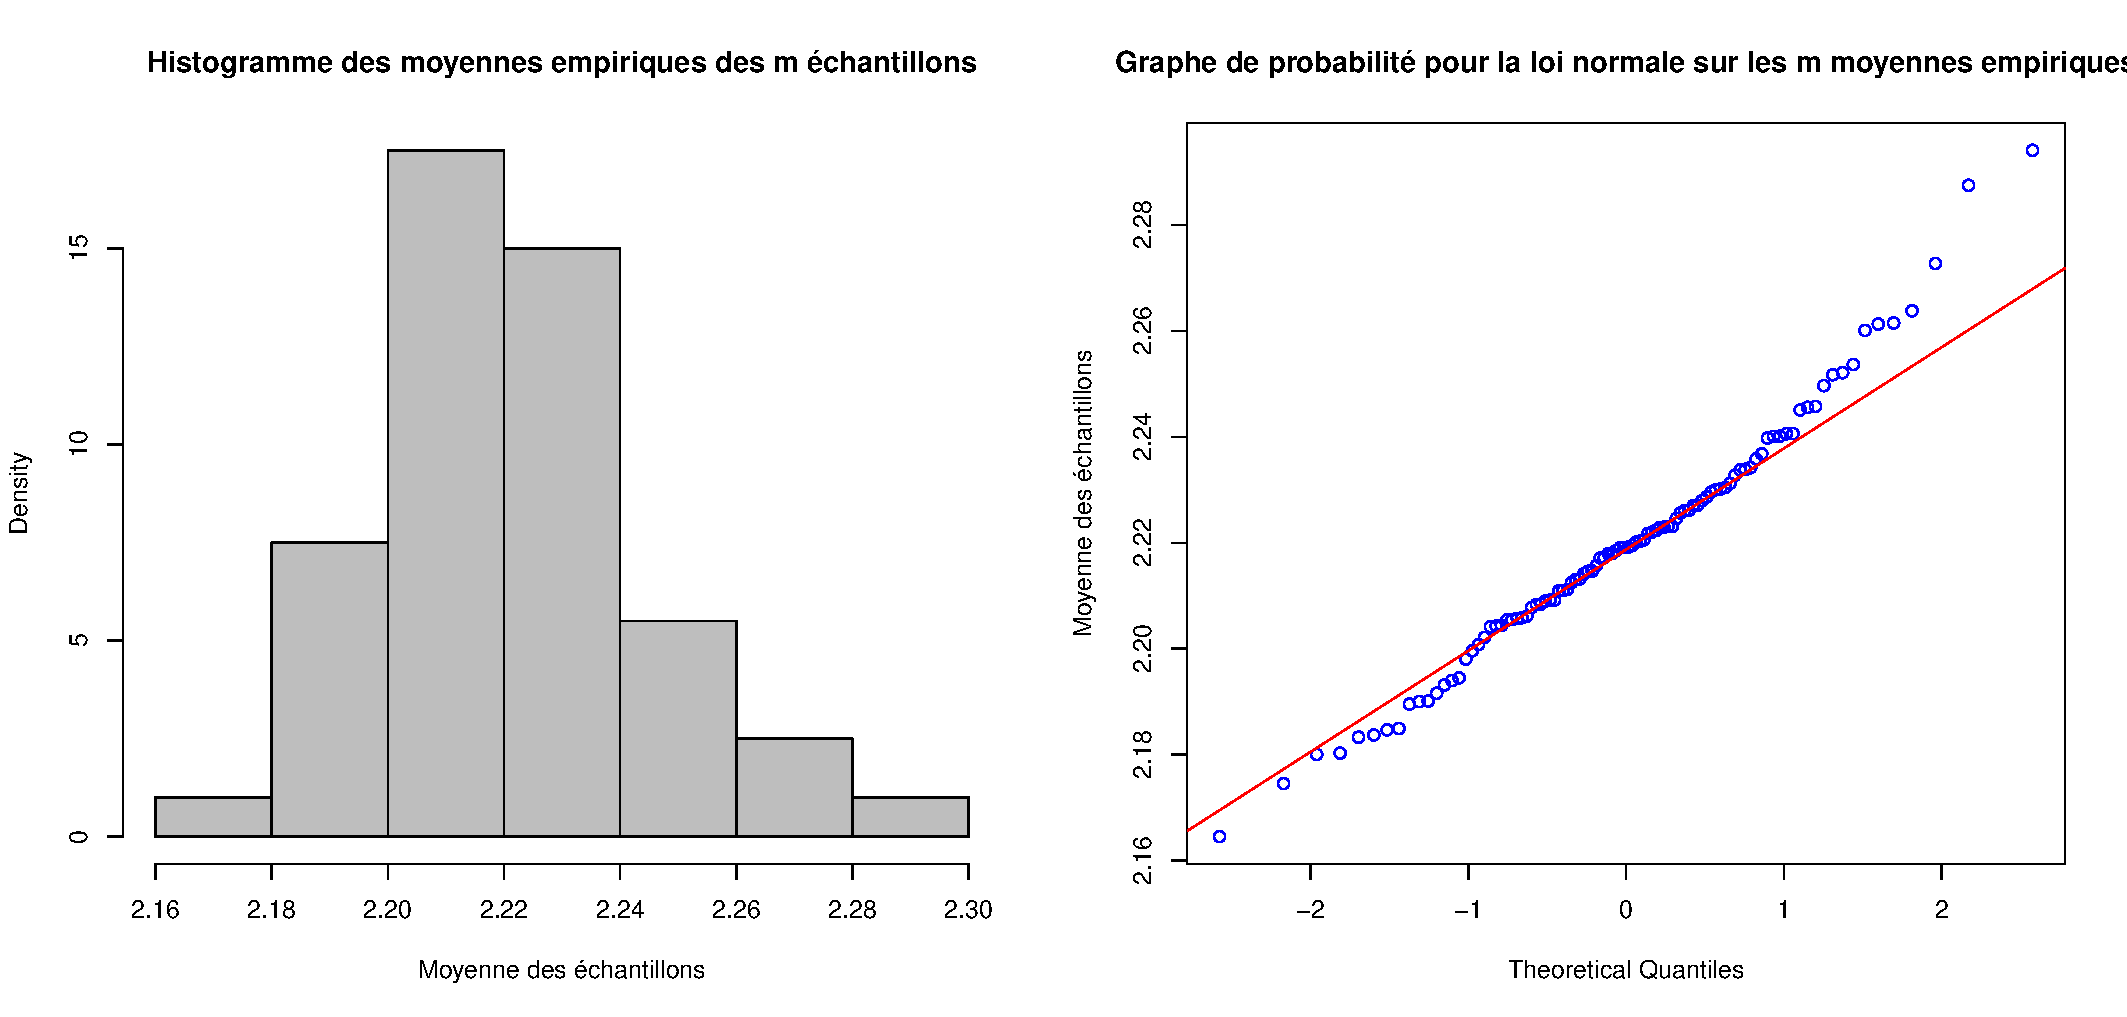
\includegraphics[width=1.0\textwidth]{figures/GraphP2Q54.pdf}
\caption{Etude de la distribution $\bar X_n$ par une distribution normale pour n=100}
\end{figure*}

\begin{figure*}[ht]
\centering
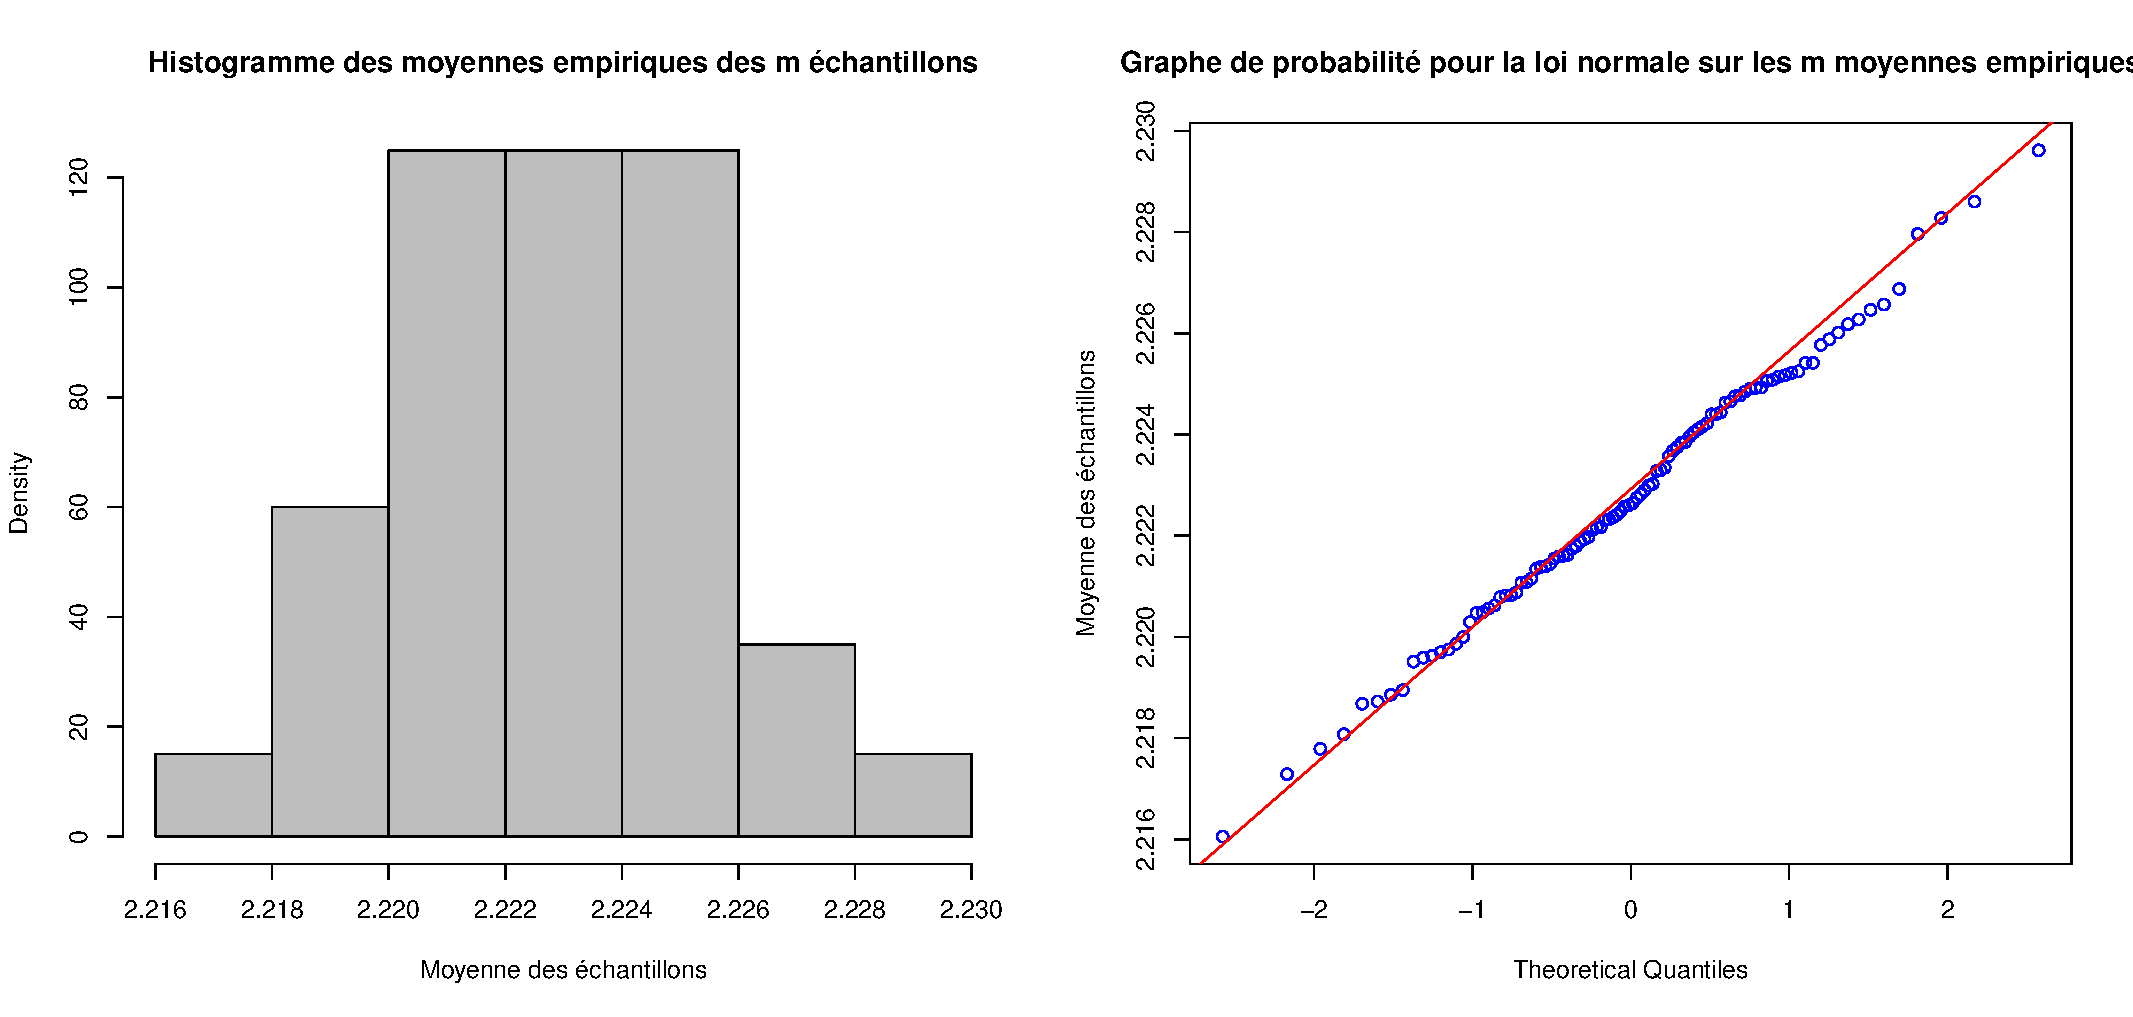
\includegraphics[width=1.0\textwidth]{figures/GraphP2Q55.pdf}
\caption{Etude de la distribution $\bar X_n$ par une distribution normale pour n=500}
\end{figure*}

\end{enumerate}
%=============
\end{document}
%=============
